
Many exciting possibilities loom on the horizon for this tool chain construction effort.  We briefly describe some forward-looking concepts currently in discussion for the tools.  %The fourth stage of development is depicted in Fig. \ref{fig:uc4}.

%\begin{figure}
%	\centering
%   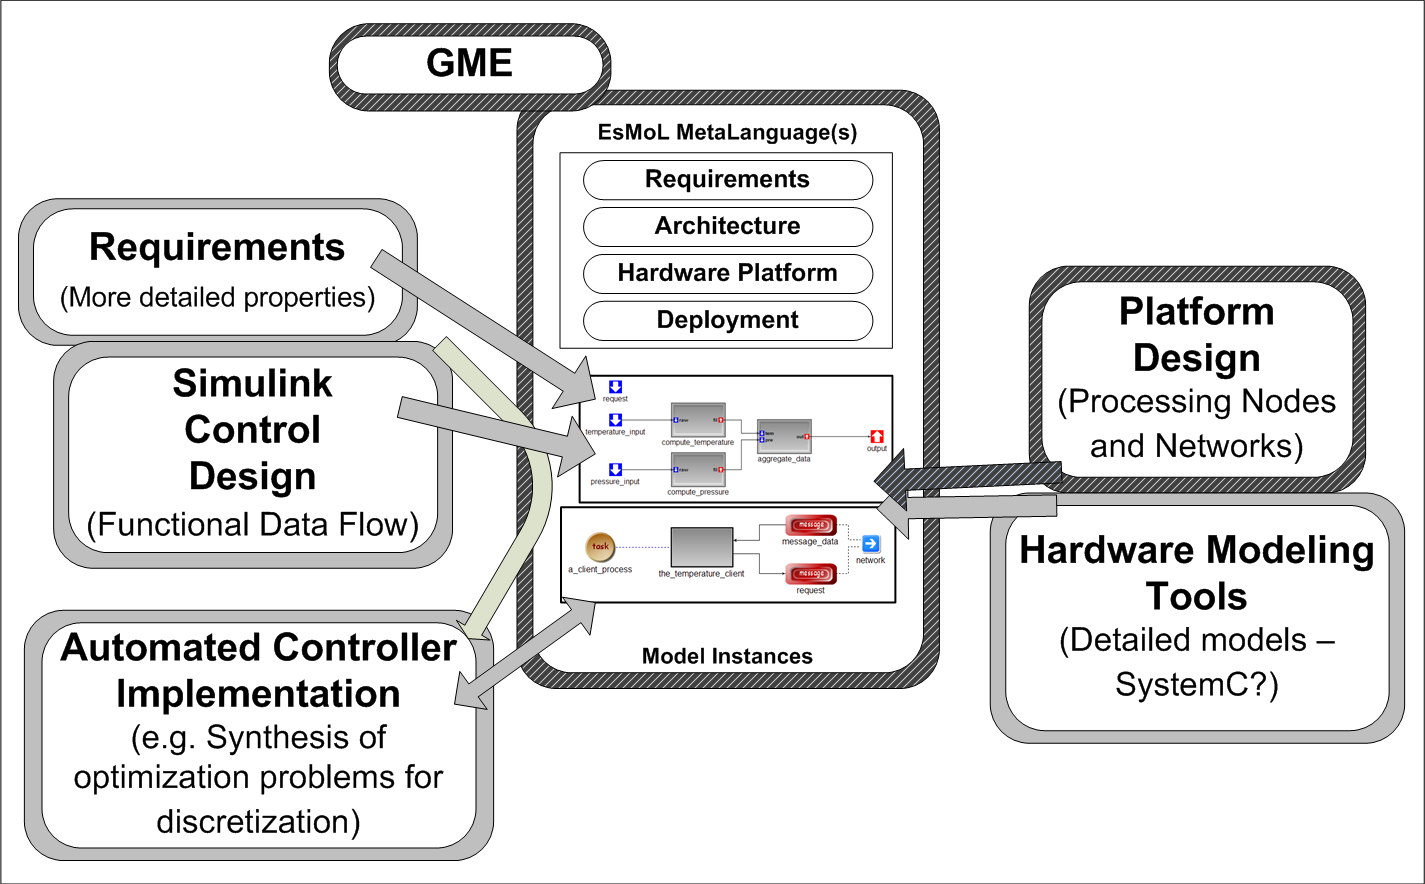
\includegraphics[width=0.55\columnwidth]{diagrams/usecase4.png}
%   \caption{Stage 4. Extension of formal requirements and platform models and automated synthesis of discretized controllers.  These are wishlist items, though some preliminary experiments and designs have been made.}
%   \label{fig:uc4}
%\end{figure}

The current modeling languages describe systems which provide performance and reliability guarantees by implementing a time-triggered model of computation.  This is not adequate for many physical processes and controller platforms.  We also need provisions for event-triggered communication and components.  Event-triggered component structures give rise to interesting and useful communication patterns common in practical systems (e.g. publish-subscribe, rendezvous, and broadcast). Several research projects have explored heterogeneous timed models of computation.  Two notable examples are the Ptolemy project~\cite{ucb:ptolemy2} and the DEVs formalism and associated implementations~\cite{DEVSpp}.  More general simulation and model-checking tools for timed systems and specifications include UPPAAL~\cite{UPPAAL} and timed abstract state machines~\cite{TASM}.  We aim to identify useful design idioms from event-triggered models and extend the semantics of the modeling language to incorporate them.  Synthesis to analysis tools is also possible using model APIs.  

Safe automation of controller implementation techniques is another focus.  Control designs are often created and simulated in continuous time and arbitrary numerical precision, and then discretized in time for platforms with periodic sampling and in value for platforms with limited numeric precision.  Recent work in optimization and control offers some techniques for building optimization problems which describe valid controller implementation possibilities~\cite{LMITrunc}~\cite{LMINetwork}. Early model interpreter work aims to generate such optimization problems directly from the models.  Other interesting problems include automated generation of fixed-point scaling for data flow designs.  If integrated, tools like BIP~\cite{BasuBozgaSifakis07} provide potential for automated verification of distributed computing properties (safety, liveness, etc...).  Model representation of data flow functions, platform precision, and safety requirements could be used together for scaling calculation.
  
The addition of proper formal requirements modeling can enable synthesis of conditions for model checking and other verification tools.  Executable semantics for these modeling languages can also provide the behavioral models to be checked (see Chen~\cite{SU_TA}~\cite{SU_MT}, Gargantini~\cite{ASM_SPIN}, and Ouimet~\cite{TASM_SAT}).  Other relevant work includes integration of code-level checking, as in the Java Pathfinder~\cite{Pathfinder} or Saturn~\cite{Stanford_Saturn} tools.  Synthesis to these models must also be verified, an active area of research at ISIS~\cite{ananth:2006}.
